\documentclass[letterpaper]{article}
\usepackage{natbib,alifexi}
\usepackage[utf8]{inputenc}
\usepackage{amsmath}
\usepackage[toc,page]{appendix}
\usepackage[frenchb]{babel}
\usepackage[T1]{fontenc}
\usepackage{placeins, latexsym, amssymb}

\usepackage[hidelinks]{hyperref}

\title{Prédiction des temps de trajet dans un réseau\\ de bus à l'aide de données historiques}
\author{Nikita Marchant$^{1}$\\
Superviseurs : Martine Labbé, Samuel Deleplanque
\mbox{}\\\\
$^1$Université Libre de Bruxelles, Département d'Informatique\\
nimarcha@ulb.ac.be}

\setlength{\parskip}{0.5em}
\begin{document}
\maketitle

\begin{abstract}

Prédire en temps-réel l'heure d'arrivée d'un véhicule de transports en commun devient de plus en plus vital dans nos vies connectées. Ce travail analyse rapidement l'état de l'art sur les méthodes statistiques et de machine learning utilisées dans la littérature. Nous proposons puis implémentons un modèle de $k$ plus proches voisins ($k$NN) pour prédire les temps de trajets des véhicules de la STIB et nous démontrons pour finir la performance de ce modèle face au modèle actuellement déployé par la STIB.

\end{abstract}

\section{Introduction}

Le but de ce projet est de pouvoir prédire, en temps réel, l'heure d'arrivée d'un véhicule de transports en commun aux arrêts de son trajet.
Dans le cadre de ce travail, la prédiction sera effectuée pour des lignes de bus,
trams et métros de la STIB\footnote{Société de transports en commun à Bruxelles (Belgique)}.

Un réseau de transport en commun est difficile à modéliser en raison de sa complexité et par le fait qu'il est très influençable par des événements stochastiques. L'approche utilisée ici ne sera non pas de modéliser le réseau pour prédire son état futur, mais d'extrapoler, grâce à des algorithmes de machine learning, les trajets des véhicules grâce à des données historiques récoltées au préalable.


\section{État de l'art}

\subsection{Méthodes naïves}

Plusieurs méthodes de prédiction naïves sont décrites dans la littérature pour servir de témoin et pouvoir comparer les performances de l'algorithme proposé par rapport aux autres méthodes [\cite{Altinkaya2013}].

La plus simple des méthodes naïves est de prédire la durée de trajet entre deux arrêts en utilisant simplement la durée spécifiée dans les horaires statiques préparés par l'opérateur de la ligne. Cette méthode ne prenant aucun aléa en compte, elle n'est évidemment pas utilisée pour de la prédiction en temps réel.

La seconde méthode, celle utilisée par la STIB, est de prédire le temps de trajet entre deux arrêts comme étant la moyenne des temps de trajets des $n$ (dans notre cas, 3) derniers véhicules de la ligne étant passés sur ce tronçon. Celle-ci donne malheureusement des résultats quasiment toujours moins bons que les autres méthodes existantes [\cite{Altinkaya2013}].

Un des points faibles de cette méthode est qu'elle est limitée par le fait qu'il faut attendre que $n$ véhicules aient subi une perturbation donnée pour qu'elle soit pleinement prise en compte pour les prédictions suivantes (et sur ce temps là, la perturbation sera peut-être finie).

Un autre problème dont souffre cette méthode est le fait qu'un bus peut se remplir fortement en une seule fois (par exemple à la sortie d'une école ou lors de la fin d'un gros événement). Celui-ci sera donc fortement ralenti à cause du temps pris à charger et à décharger ses passagers alors que le modèle prédira qu'il sera aussi rapide que les véhicules précédents.

De plus, les véhicules qui suivent celui qui est retardé seront prédits en retard alors qu'ils risquent même d'être en avance, ayant moins de passagers à embarquer et à débarquer.

Il existe aussi des méthodes hybrides comme celle présentée dans \cite{lin1999experimental} qui utilisent la position GPS, l'horaire statique ainsi que le retard calculé pour prédire l'heure d'arrivée. Celles-ci nécessitent des données plus précises et d'une meilleure résolution, mais donnent aussi de meilleurs résultats.



\subsection{Vitesse moyenne}

Comme le modèle hybride présenté ci-dessus, d'autres modèles exploitent le fait que certaines compagnies équipent leurs véhicules de systèmes qui émettent en continu leur position GPS ainsi que leur vitesse. La position du véhicule n'étant évidement pas infiniment précise, il faut donc ensuite utiliser des techniques de \textit{map-matching} : faire correspondre le trajet mesuré au trajet prévu, sur une carte, afin de connaître sa ``vraie'' position.

Il est ensuite éventuellement possible de transformer cette position, en deux dimensions, en une position unidimensionnelle : la distance parcourue sur la ligne depuis le terminus; pour simplifier les algorithmes de prédiction.

Grâce à ces informations, il est possible d'estimer la vitesse du véhicule. La vitesse instantanée pouvant être nulle et donc prédire un temps d'attente infini, nous ne pouvons pas l'utiliser directement.

Pour cela, \cite{Maciver2002} combine la vitesse moyenne (calculée à l'aide des mesures précédentes) avec la vitesse instantanée rapportée par le véhicule. Le temps restant jusqu'à l'arrêt suivant est ensuite estimé comme la distance restant à parcourir multipliée par cette vitesse.


\subsection{Filtres de Kalman}

Les filtres de Kalman, développés initialement pour estimer la position d'objets détectés par des radars [\cite{kalman1960new}] sont utilisés couramment dans la littérature [\cite{wall1999algorithm, cathey2003prescription, shalaby2004prediction}] pour estimer la position ainsi que l'état (principalement la vitesse) de véhicules sur le réseau afin de filtrer et lisser les mesures bruitées reçues depuis les véhicules.

De plus, les filtres de Kalman peuvent aussi être utilisés pour de la prédiction. \cite{cathey2003prescription} étaient les premiers à le faire pour prédire des temps d'arrivée de transports en commun. En effet, ces filtres peuvent être utilisés pour lisser un signal (en estimant l'état dans le passé), filtrer (dans le présent) ou prédire (en estimant l'état futur).

Ceux-ci ont été suivis par beaucoup d'autres (voir \cite{yang2005travel, Altinkaya2013}).

\cite{cathey2003prescription} ont montré que les résultats obtenus grâce à cette méthode étaient meilleurs que les modèles basés sur des moyennes historiques et que ceux utilisant la régression. Cependant, ceux-ci ne prennent en compte qu'un trajet à la fois et ne profitent pas des données historiques pour apprendre des comportements récurrents.

\subsection{$k$ plus proches voisins}

La méthodes des $k$ plus proches voisins\footnote{$k$-nearest neighbors ou encore $k$-NN.} est une méthode largement utilisée dans le domaine des transports publics. Celle-ci est basée sur le fait que les trajets des véhicules sont influencés par un grand nombre de facteurs difficiles à prédire. Néanmoins, il est possible de chercher dans le passé des trajectoires similaires à la trajectoire à prédire. Dans de nombreux cas, ces trajectoires passées ont été soumises aux mêmes aléas que la trajectoire actuelle. Leur comportement peut donc être utilisé pour tenter de prédire le trajet futur. [\cite{tiesyte2008similarity}]

Il est nécessaire de déterminer quelles caractéristiques d'un trajet seront utilisées lors du calcul de la similarité entre deux trajets. \cite{baker2014predicting} utilisent par exemple la position le long de la ligne, la latitude, la longitude, l'instant présent, le jour de la semaine, l'heure du jour, le numéro de séquence du bus ainsi que la déviation par rapport à l'horaire, alors que \cite{tiesyte2008similarity} n'utilisent que la position le long de la ligne.

Le nombre de variantes de ce modèle étant assez élevé, il est difficile d'en évaluer sa performance. Il semble par contre assez clair que celui-ci est plus performant que les méthodes naïves.

\subsection{Réseaux de neurones}

Les réseaux de neurones sont de plus en plus populaires dans la communauté du machine learning depuis que la capacité de calcul des ordinateurs modernes permet des implémentations rapides. Ceux-ci sont composés de neurones et de synapses. Habituellement, les neurones sont disposés par couches. Chaque neurone est relié grâce aux synapses à chaque neurone de la couche précédente et suivante. Les données d'entrées sont fournies à la première couche et ces données sont ensuite propagées à travers les synapses ainsi que les neurones jusqu'à la couche de sortie qui est utilisée comme prédiction.

Chaque neurone dispose d'une fonction d'activation et chaque synapse d'un poids, il donc est intéressant d'essayer d'optimiser ceux-ci pour que la sortie produise une bonne prédiction. Cette opération s'appelle l'apprentissage : pendant cette période, l'algorithme utilise l'ensemble d’entraînement comme entrée et pour chaque vecteur de celui-ci, il produit une prédiction. Le réseau est ensuite modifié à chaque tour en fonction de l'erreur pour essayer de diminuer celle-ci petit à petit.

Les réseaux de neurones sont fort appréciés pour leur capacité à découvrir des relations complexes et non linéaires entre des variables. Cela en fait de bons candidats dans le cas de prédictions de temps de trajet. [\cite{Chen2004}]

Leur désavantage est le fait qu'il est assez difficile, délicat et encore coûteux computationnellement de faire converger le réseau vers un état optimal. [\cite{Altinkaya2013}]


\section{Méthode développée}

Tous les réseaux urbains étant différents, les méthodes décrites dans l'état de l'art ne sont pas directement applicables à notre cas d'étude : le réseau de la STIB. Dans notre cas, nous ne disposons ni de trace GPS, ni d'information sur le taux de remplissage des véhicules ni même de leur numéro de séquence, ce qui élimine déjà une partie des méthodes présentées ci-dessus.

Il semble que la tendance actuelle est de plus en plus d'utiliser des modèles hybrides, mélangeant plusieurs techniques pour prendre les avantages de chacune. Nous proposons donc ici d'utiliser ici une méthode de collection de données originale, couplée à une prédiction à l'aide de la méthode des $k$ plus proches voisins et nous finirons par suggérer des améliorations à apporter à cette approche.

L'implémentation a été découpée en 5 grandes parties : premièrement, la collection de données pour alimenter l'apprentissage du modèle, ensuite le traitement de ces données pour améliorer leur qualité et les transformer en un format utilisable par le modèle, l'étape suivante a été l'analyse et le choix de fonctions de score pour entraîner le modèle et pour finir, l’entraînement en lui même ainsi que l'analyse des résultats.

\subsection{Collection des données}

La STIB ne mettant pas à disposition ses données historiques, il a fallu commencer par récolter des informations grâce à un programme écrit pour l'occasion.

Les deux seules sources de données sur l'état du réseau en temps réel disponibles sur internet sont :
\begin{itemize}
    \item pour chaque ligne, la position précise à un arrêt près de chaque véhicule,
    \item pour chaque arrêt, une estimation du temps d'attente avant le prochain véhicule de chaque ligne.
\end{itemize}
\vspace{0.5em}
La source de données qui a été choisie est la première pour deux raisons : le réseau de la STIB disposant de milliers d'arrêts, il aurait été difficile de récolter avec une fréquence suffisante les temps d'attente pour chaque arrêt. De plus, les temps d'attentes étant eux mêmes des prédictions, il serait un peu illogique de les utiliser comme des mesures.

La source choisie souffre tout de même d'un problème non-négligeable : les véhicules apparaissent sur la ligne comme de simples point non identifiés. Il n'est donc pas possible de récupérer le numéro du véhicule, sa plaque d'immatriculation ou tout autre identifiant unique. De plus, si deux véhicules d'une même ligne sont suffisamment proches, leurs images se confondent et ils n'apparaissent plus que comme un seul point.

Le processus de collection des données est un programme \textit{Python3} utilisant \texttt{aiohttp} pour permettre d'effectuer des requêtes HTTP asynchrones au serveur web de la STIB et ainsi permettre une période d’échantillonnage de 20 secondes pour chaque ligne, dans chaque sens (ce qui fait 142 mesures toutes les 20 secondes dans l'état actuel du réseau).

La période a été choisie arbitrairement car une fréquence plus élevée imposait une charge trop lourde au serveur de la STIB et une fréquence plus faible aurait été trop imprécise.

Cette collection de données a permis l'enregistrement d'approximativement 80 millions de mesures en 6 mois, réparties sur l'ensemble des lignes.


\subsection{Traitement des données}

Les données récupérées grâce à la méthode décrite dans la section précédente sont malheureusement de mauvaise qualité. En effet, il est courant qu'un véhicule cesse d’émettre sa position pendant plusieurs minutes, que la source de donnée tombe en panne ou que les positions de deux véhicules fort proches soient confondues en un seul point.

De plus, les mesures ne sont pas directement utilisables par l'algorithme que nous avons choisi. En effet, nous ne disposons que d'une suite de positions (les sorties de notre programme de mesure sont des vecteurs horodatés de booléens, voir annexe) et ce dont nous avons besoin sont les durées que chaque véhicule a pris pour parcourir les distances entre deux arrêts consécutifs.

Nous avons donc développé un algorithme qui assigne un identifiant à chaque nouveau point (ou véhicule) qui apparaît sur une ligne et qui, lors des mesures suivantes essaye dans la mesure du possible de détecter si un point est déjà connu et qu'il s'est déplacé durant l’intervalle ou si c'est un nouveau point (par exemple un bus qui vient du dépôt et qui est injecté sur la ligne).

Grâce à ces identifiants uniques que nous générons, nous pouvons reconstituer des trajets, définis comme une suite de paires <position, instant> pour chaque véhicule que nous avons détecté. Cela est possible en parcourant simplement les mesures traitées et en enregistrant la position de chaque identifiant dans la ligne à chaque instant.

Dans l'optique de pouvoir proposer des prédictions en temps réel, l'algorithme supporte un mode dans lequel il a connaissance des trajets passés et non terminés (dont le véhicule n'est pas arrivé au terminus) et qui permet de compléter ces trajets au fur et à mesure que de nouvelles mesures sont disponibles.

L'algorithme, bien qu'ayant pris du temps à développer et à paramétrer ne présente pas de grand intérêt scientifique et est donc détaillé en annexe.



\subsection{Modèle d'apprentissage: les $k$ plus proches voisins}

L'algorithme des $k$ plus proches voisins
est une méthode d'intelligence artificielle qui peut être utilisée aussi bien pour de la classification que pour de la régression [\cite{trevor2009elements}].
L'idée de cette méthode est de trouver les $k$ trajets les plus similaires à la cible et d'utiliser ceux-ci pour extrapoler le temps de trajet futur.

Pour calculer la similarité entre deux trajets, nous devons extraire des \textit{features}, des grandeurs qui caractérisent ces trajets. Les features que nous utiliserons ici sont les temps que le véhicule a pris pour voyager entre deux arrêts.

Un trajet n'est évidemment pas caractérisé uniquement par ces grandeurs mais nous verrons qu'en première approximation ces grandeurs sont déjà suffisantes \footnote{Une autre feature très intéressante et fort utilisée dans la littérature est la taux de remplissage du véhicule mais nous n'avons pas accès à cette donnée dans notre cas. D'autres features qui pourraient être intéressantes sont énumérées dans les perspectives, en fin d'article}.

Nous commençons donc par projeter chaque trajet dans un espace à $n$ dimensions avec $n+1$ étant le nombre d'arrêts déjà effectués par le véhicule $\alpha$ (celui dont on cherche à prédire le temps de trajet futur).

Les trajets sont représentés par le vecteur colonne
$T_{\beta} = \begin{pmatrix}d_{1,\beta}, d_{2,\beta}, ..., d_{n,\beta}\end{pmatrix}^{T}$
avec $d_{i,\beta}$ étant la durée du trajet entre l'arrêt $i$ et $i+1$ pour le véhicule $\beta$.

Maintenant que nous avons transformé nos trajets en vecteurs, nous pouvons utiliser tous les trajets du passés (l'ensemble d'apprentissage) et les placer dans cet espace à $n$ dimensions pour entraîner notre algorithme.

Une fois que l'algorithme est entraîné, nous pouvons faire une prédiction pour un trajet dont la fin est inconnue ($\alpha$). Pour cela, nous le plaçons aussi dans cet espace et nous mesurons sa similarité par rapport à tous les autres trajets de l'ensemble d'apprentissage.

La similarité $s_{\beta,\gamma}$ (ou distance) entre deux trajets $\beta$ et $\gamma$ est définie comme la distance euclidienne entre deux vecteurs :

\begin{eqnarray}
s_{\beta,\gamma} = \sqrt{\sum_{j=0}^{n}(d_{j,\beta} - d_{j,\gamma})^2}
\end{eqnarray}

Nous sélectionnons ensuite les $k$ vecteurs dont la similarité est la plus proche de $\alpha$ et nous nommons cet ensemble $\mathcal{V}$ : les plus proches voisins.

Dans la version originale de $k$NN, la prédiction du temps de trajet $\hat{d}_{n+i,\alpha}$ est ensuite donnée par la moyenne des temps de trajets pour les vecteur appartenant à $\mathcal{V}$.

\begin{eqnarray}
\hat{d}_{n+i,\alpha} = \frac{1}{k} \sum_{v \in \mathcal{V}}d_{n+i,v}
\end{eqnarray}

Il est aussi possible d'effectuer la régression à l'aide d'une moyenne pondérée. Chaque vecteur est pondéré par l'inverse de sa distance par rapport au vecteur cible :

\begin{eqnarray}
\hat{d}_{n+i,\alpha} = \sum_{v \in \mathcal{V}} s_{\alpha, v} \cdot \frac{1}{k} \sum_{v \in \mathcal{V}}( \frac{d_{n+i,v}}{s_{\alpha, v}})
\end{eqnarray}

La projection des trajets dans un espace à $n$ dimension ainsi que l'implémentation de l'algorithme des plus proches voisin ont dans un premier temps été écrits en \textit{Python3}, uniquement à l'aide de la librairie \texttt{numpy} pour faciliter les calculs vectoriels et un prototypage rapide. Dans un second temps, nous avons utilisé la librairie \texttt{scikit-learn} pour profiter de son implémentation optimisée de $k$NN.

\section{Fonctions de score}

Afin d'effectuer un bon choix de l'hyper-paramètre $k$ ainsi que de choisir entre la moyenne pondérée ou non, il est important de pouvoir comparer deux modèles entre eux. Pour cela, nous aurons aussi besoin d'assigner un score à une prédiction. Ce score sera établi en fonction de la différence entre la prédiction et sa réalisation.

\subsection{Score d'une prédiction}
Pour assigner un score à une prédiction, la littérature utilise souvent le RMSE\footnote{Root Mean Squared Error}: l'erreur quadratique moyenne.
Cependant, cette métrique souffre d'un problème :
qu'un bus soit annoncé une minute à l'avance ou une minute en retard est pondéré de la même manière alors que dans un cas l'usager attend son bus une minute de plus et que dans l'autre il le rate, ce qui est plus grave.

Nous avons donc implémenté d'autres métriques qu'il nous semblait intéressant de pouvoir minimiser à fin d'en choisir une :
\begin{itemize}
    \item Le RMSE double négatif : chaque erreur négative (quand un bus est annoncé plus tard qu'en vrai) est doublée et en suite on applique le RMSE.
    \item RMSE pondéré linéairement : l'erreur de prédiction pour l'arrêt suivant est pondéré avec un poids de 5, l'erreur pour le dernier arrêt est pondérée avec un poids de 1 et les arrêts entre les deux sont pondérés linéairement entre 1 et 5.
    \item RMSE pondéré exponentiellement : l'erreur de prédiction pour le $n$ème arrêt suivant est pondéré avec un poids de $\frac{1}{n}$
\end{itemize}
\vspace{1em}

La première métrique résout (ou en tout cas diminue) le problème du bus raté et les deux suivantes prennent en compte le fait qu'il est plus intéressant de bien prédire le futur proche et un peu moins bien le futur lointain que de bien prédire l'entièreté du trajet.

Pour comparer ces différentes métriques, nous entraîné un $k$NN avec un $k$ fixé arbitrairement à 130 à l'aide de 12000 trajets de la ligne de bus 95 vers Grand-Place en utilisant les 10 premiers arrêts comme donnée connue et les 13 suivants comme donnée à prédire. Ensuite, nous avons effectué 6000 prédictions pour d'autres trajets de la même ligne et nous avons calculé leur score avec chaque métrique.

\begin{figure}[h]
   \centerline{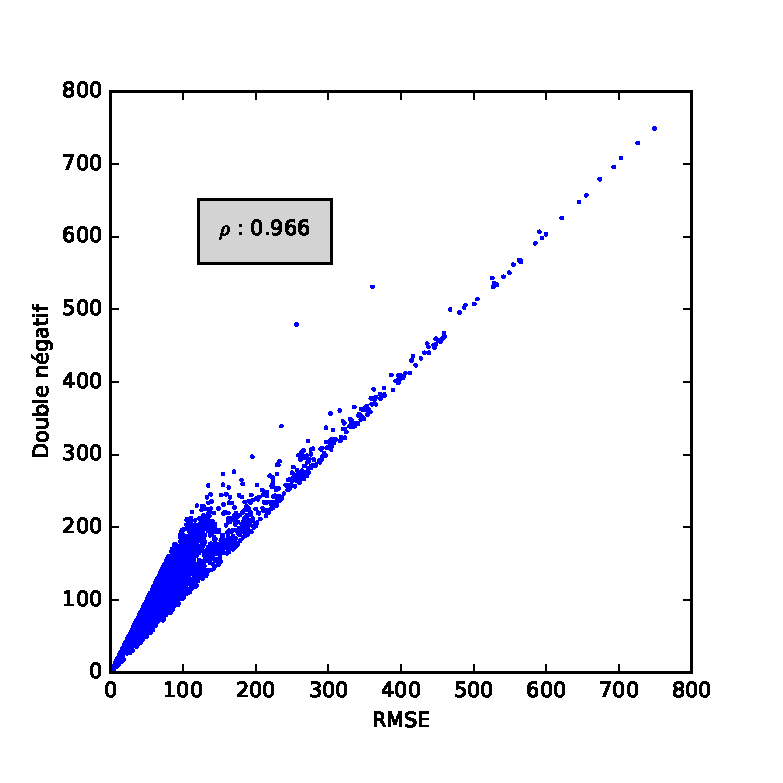
\includegraphics[width=9cm]{metrics.eps}}
   \caption{\label{fig:rmse-vs-double}Comparaison entre le RMSE et le double négatif pour chacune des prédictions.}
\end{figure}

Nous avons ensuite comparé graphiquement deux à deux chacune des fonctions de score sur l'ensemble des 6000 prédictions. Nous pouvons en voir un exemple dans la figure~\ref{fig:rmse-vs-double} : chaque point représente une prédiction avec, en abscisse son score selon le RMSE et en ordonnée son score selon le RMSE double négatif. Des graphes pour toutes les autres comparaisons se trouvent en annexe.

Cette première comparaison nous a déjà permis d'apercevoir une corrélation linéaire entre les différentes fonctions.
En plus de cette corrélation déterminée visuellement, nous avons comparé la corrélation de rang entre les fonctions grâce au coefficient de corrélation de Spearman (ou $\rho$). Celui-ci nous donne un indice sur le fait que deux fonctions ordonnent un ensemble de la même manière\footnote{En effet, il nous importe peu que la corrélation soit linéaire ou même quadratique : tant qu'on peut classer les prédiction de la meilleure à la moins bonne et que ce classement ne change pas lors d'un changement de fonction de score, cela est suffisant pour nous.}. Celui-ci varie entre -1, quand l'ordre est parfaitement inversé à 1, quand l'ordre est identique.

Sa formule est définie comme ceci, $d_i$ étant la différence entre le rang de l'élément $i$ défini par la première fonction et la seconde :

\begin{eqnarray}
\rho = 1 - \frac{6 \sum_{i=1}^{n} d^2_i}{n^3 - n}
\end{eqnarray}

\begin{table}[h]
\centering
\begin{tabular}{|l|c|c|c|c|}
  \hline
  & RMSE & linéaire & exponentiel & double \\
  \hline
RMSE & 1.000 & 0.961 & 0.812 & 0.966 \\
linéaire & 0.961 & 1.000 & 0.896 & 0.926 \\
exponentiel & 0.812 & 0.896 & 1.000 & 0.793 \\
double & 0.966 & 0.926 & 0.793 & 1.000 \\
  \hline
\end{tabular}
  \caption{\label{tab:rho} Rho de Spearman entre chaque chaque paire de métrique de score.}
\end{table}

Le RMSE double négatif semblant être la métrique la plus intéressante à minimiser pour les utilisateurs et le RMSE simple étant quasiment identique (voir table \ref{tab:rho} et figure \ref{fig:rmse-vs-double}), nous avons choisi d'utiliser par la suite le RMSE pour sa simplicité d'implémentation et sa rapidité (ce n'est que la norme du vecteur d'erreur, fonction qui est déjà implémentée efficacement dans \texttt{numpy})

\FloatBarrier
\subsection{Score d'une modèle}

Maintenant que nous savons comparer et donner un score à des prédictions, nous pouvons choisir une technique pour scorer un modèle en entier, ce qui nous permettra entre autres de choisir l'hyper-paramètre $k$ et de choisir entre le $k$NN pondéré ou non.

Pour cela, nous devons agréger d'une manière ou d'une autres toutes les prédictions qu'un modèle a fait pour un ensemble de départ. Ici le choix des fonctions d’agrégation score ont été assez simples. Nous avons comparé la moyenne, la médiane ainsi que le maximum de l'ensemble des scores des prédictions du modèle.

Pour cela, nous avons réutilisé le même set de données que dans la section précédente mais cette fois ci en faisant varier $k$ de 1 à 1000 en 20 incréments\footnote{Nous avons peu d’échantillons par rapport à la comparaison précédente car il est coûteux computationnellement de créer, entraîner et scorer des centaines de modèles.}.

Nous avons remarqué une corrélation assez forte, 0.822, entre la médiane et la moyenne ainsi qu'une absence totale de corrélation entre le maximum et les deux autres (0.007 et 0.180).

Cela semblerait s'expliquer par le fait que même si un modèle est très précis la plus part du temps, il fera tout de même au moins une prédiction avec une erreur significativement grosse et que cette erreur est bornée supérieurement par la distance entre le trajet le plus lent et le plus rapide.

Au vu de la faible différence entre la moyenne et la médiane, mous avons arbitrairement choisi d'utiliser la moyenne comme fonction d'agrégation de scores.

\subsection{Entraînement et choix des paramètres}

Une fois les méthodes de score déterminées, nous pouvons choisir expérimentalement une valeur pour l'hyper-paramètre $k$ en cherchant à minimiser le score de notre modèle.

Pour éviter l'\textit{overfitting} (en français le sur-apprentissage), le fait qu'un modèle donne des résultats artificiellement bons pour l'ensemble d’entraînement au détriment de bonnes prédictions pour de nouveaux échantillons, nous avons utilisé la méthode de la validation croisée.

La validation croisée (ou plus communément \textit{cross-validation}) est une technique qui permet d'estimer la fiabilité d'un modèle grâce à un échantillonnage des données. Nous avons utilisé la méthode \textit{testset validation} pour des raisons de complexité computationnelle.

Cette méthode fonctionne de la manière suivante : l'ensemble des trajets divisé en deux échantillons, l'un contenant $2/3$ des données et le second contenant le dernier tiers. Le premier devient l'ensemble d'apprentissage et sert uniquement à entraîner le modèle alors que le second devient l'ensemble de test et dont les prédictions serviront à scorer le modèle.

Cet échantillonnage étant fait, nous voyons empiriquement que quand $k$ augmente, le score d'un modèle diminue de manière presque continue jusqu'à atteindre le $k$ optimal puis se mets à augmenter une fois ce point dépassé.

Au lieu d'itérer sur l'entièreté des valeurs raisonnables de $k$ (par exemple l’intervalle $[1,1000]$) pour trouver la valeur minimale de $f(k)$, nous avons utilisé la méthode de Brent, décrite dans \cite{rivlin1973algorithms} et implémentée dans \texttt{scipy} qui permet de minimiser une fonction dont l'expression analytique (et donc la dérivée) n'est pas connue.

Nous avons utilisé la méthode de Brent avec un nombre d'itérations limité à 40 et dont la convergence est considérée comme atteinte quand l'erreur relative est inférieure à 0,1.

Les résultats que nous avons obtenu sont des $k$ variant entre 100 et 800, selon les lignes. Le fait que c'est intervalle soit si large semble s'expliquer par le fait que chaque ligne à une fréquence différente et que par exemple, pour une ligne importante comme le 95 nous disposons de plus de 35000 trajets alors que pour une ligne à faible fréquence comme le 41 nous ne disposons que de 8000 trajets\footnote{Les mesures dont nous disposons pour les lignes à haute fréquence sont aussi de moins bonne qualité (il y a plus de chances que notre algorithme confonde deux véhicules ou ne détecte pas un dépassement quand les véhicules sont proches les uns des autres).}.

Nous avons ensuite effectué la même recherche de l'hyper-paramètre $k$ pour la version pondérée par la distance de $k$NN. Celle-ci a retourné approximativement les les mêmes $k$ optimaux, cependant la valeur de la fonction de score était systématiquement égale ou inférieure à la version non pondérée. Dans le cas de la ligne du 95, nous avons été jusqu'à constater un score deux fois meilleur pour la version pondérée.

\section{Résultats}

Le choix d'un hyper-paramètre permettant de minimiser l'erreur de prédiction nous permet donc maintenant de comparer nos prédictions faites à l'aide d'un $k$NN à celles faites par la STIB avec la méthode de la moyenne des trois derniers trajets.

Pour cela, nous avons utilisé la même méthode d'échantillonnage que précédemment. Nous avons donc entraîné notre modèle avec $2/3$ des données et effectué des prédictions sur le tiers restant (l'ensemble de test). Ensuite, pour chaque trajet de l'ensemble de test, nous cherché les trois trajets précédents dans le temps (qu'ils appartiennent à l'ensemble de test ou non) pour en faire la moyenne et l'utiliser comme la prédiction que la STIB aurait faite.

Les résultats démontrent l'efficacité de la méthode employée : pour certaines lignes, notre modèle prédit mieux que la STIB dans 76\% des cas.

\begin{table}[h]
\centering
\begin{tabular}{|l|c|c|c|c|c|c|}
  \hline
              &      5 &    41 &    95 & 65    & 4     \\
  \hline
  meilleur    &  76\%  & 70\%  & 63\%  & 51\%  & 70\%  \\
  2x meilleur &  10\%  & 16\%  & 12\%  & 26\%  & 14\%  \\
  2x pire     &  0.5\% & 0.6\% & 0.8\% & 3.2\% & 1.1\% \\
  \hline

\end{tabular}
  \caption{\label{tab:perf}Taux de réussite de notre modèle en fonction de la performance désirée selon les lignes}
\end{table}


De plus, on peut remarquer que lorsque que notre modèle se trompe plus que la STIB, ce n'est que de peu : $k$NN effectue une prédiction deux fois moins bonne que la STIB seulement dans 0.5\% des cas pour la ligne 5 (contre 10\% des cas pour des prédictions 2 fois meilleures). On peut observer\footnote{Des résultats pour d'autres lignes ainsi que d'autres visualisations de ceux-ci peuvent être trouvés en annexe} ce phénomène dans le tableau \ref{tab:perf} pour certaines valeurs cibles ou de manière dans la figure \ref{fig:heatmap}.


\begin{figure}[h]
   \centerline{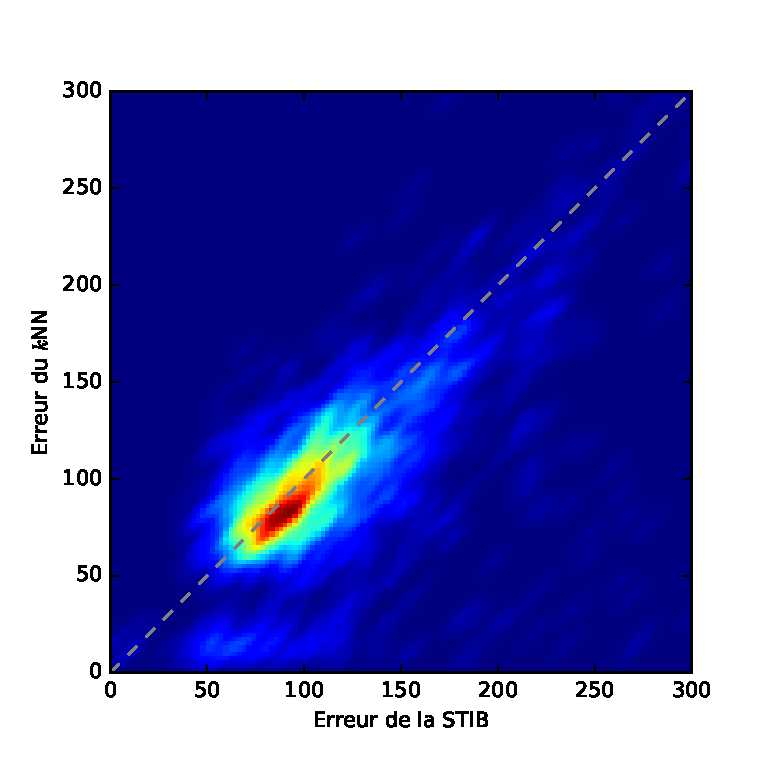
\includegraphics[width=9cm]{error-heatmap.eps}}
   \caption{\label{fig:heatmap} Estimation de la densité des trajets en fonction des erreurs de leurs prédictions selon le $k$NN ou la STIB pour la ligne 95. La ligne pointillée représente une erreur identique pour les deux modèles.}
\end{figure}

Nous pouvons aussi observer ce phénomène de manière différente en graphant (voir figure \ref{fig:density} en annexe) la densité du nuage de points par rapport à la distance qui les sépare de la sécante. Nous pouvons y voir que la grande majorité des prédictions ``ratées''\footnote{dont le score est inférieur à celui de la prédiction faite par la STIB} et qui sont donc au dessus de la sécante dans le nuage de points sont très rapprochées de celle-ci alors que la densité des prédictions réussies est plus étalée ce qui montre encore une fois, la supériorité de notre algorithme par rapport à la méthode naïve.


\section{Conclusion et perspectives}

Ce projet m'a permis d'apprendre énormément dans le domaine du machine learning ainsi que de proposer un modèle meilleur que l'actuel à la STIB pour leur prédiction en temps réel.

Ce travail pourrait être continué et amélioré en explorant d'autres méthodes d'apprentissage automatique comme les réseaux de neurones ou la régression à l'aide de noyaux.

En restant dans le domaine des $k$ plus proches voisins. Plusieurs pistes sont explorables :
\begin{itemize}
    \item actuellement notre modèle ne prend en compte que les temps de trajet entre les arrêts dans le passé pour chaque bus.
Il serait intéressant d'ajouter d'autres variables comme la distance du bus par rapport au bus qui le précède, l'heure de la journée, le jour de la semaine, le type de jour (férié, vacances, ...), des variables météorologiques, la longueur des embouteillages dans la ville,~...
    \item Il serait aussi intéressant d'essayer de pondérer les différentes dimensions de manière différente afin de mesurer l'impact de chacune. En effet, il est sûrement plus intéressant de comparer des véhicules en fonction de leur temps de trajet vers leur dernier arrêt plutôt que de leur premier.
\end{itemize}
\vspace{1em}

Pour finir, il serait aussi intéressant d'améliorer la qualité et la précision des données en entrée de l'algorithme, que ce soit par une meilleure imputation des données manquantes ou par une source de meilleure qualité car il y a de fortes chances que des données de meilleure qualité permettent des prédictions plus justes.

\section{Remerciements}

Je souhaite remercier mes superviseurs, Martine Labbé et Samuel Deleplanque pour m'avoir orienté et conseillé lors de la réalisation de ce travail.

Je souhaite aussi remercier mes amis, Romain Fontaine, Pierre Gérard et Titouan Christophe et mon père, Thierry Marchant qui m'ont prodigué de précieux conseils ce que soit pour l'algorithme de détection de trajet, pour des techniques de machine learning, des statistiques ou pour leur oreille attentive.

\footnotesize
\bibliographystyle{apalike}
\bibliography{example}


\newpage
\begin{appendices}
\section{Algorithmes de traitement et de collection de données}
\subsection{Source de données}
\label{align}
Notre source primaire de donnés se présente comme ceci :

\begin{figure}[h]
   \centerline{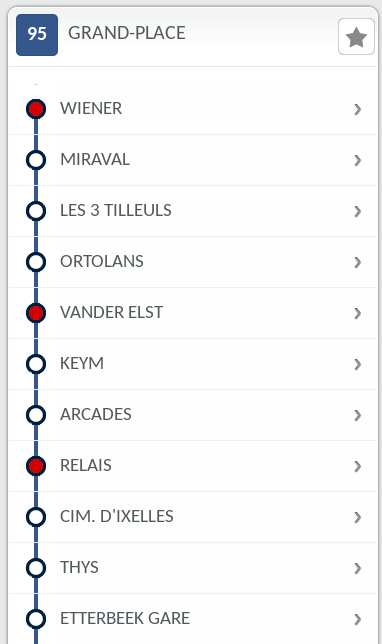
\includegraphics[width=3cm]{mstib.png}}
\end{figure}

Chaque point rouge représentant au minimum un véhicule (mais parfois plus dans le cas ou ils seraient trop proches les uns des autres). La mesure correspondant à cette copie d'écran serait ceci (un vecteur de booléens) : \texttt{[vrai, faux, faux, faux, vrai, faux, faux, vrai, faux, faux]}


\FloatBarrier
\subsection{Problèmes rencontrés}

Une fois empilés les uns au dessus des autres, ces vecteurs donnent parfois des résultats forts mauvais, comme ces mesures-ci de la ligne du 95 :

\noindent\texttt{12:10:49} $\blacksquare\square\square\square\blacksquare\square\square\blacksquare\square\square\square\square\square\square\blacksquare\square\blacksquare\square\square\square\square\square\blacksquare\square$
\texttt{12:11:09} $\blacksquare\square\square\square\blacksquare\square\square\blacksquare\blacksquare\square\square\square\square\square\blacksquare\square\blacksquare\square\square\square\square\square\blacksquare\blacksquare$
\texttt{12:11:29} $\blacksquare\square\square\square\blacksquare\square\square\blacksquare\square\blacksquare\square\square\square\square\square\blacksquare\square\blacksquare\square\square\square\square\blacksquare\blacksquare$
\texttt{12:11:49} $\blacksquare\blacksquare\square\square\blacksquare\square\square\blacksquare\square\blacksquare\square\square\square\square\square\blacksquare\square\blacksquare\square\square\square\square\blacksquare\blacksquare$
\texttt{12:12:09} $\blacksquare\blacksquare\square\square\blacksquare\square\square\blacksquare\square\blacksquare\square\square\square\square\square\blacksquare\square\blacksquare\square\square\square\square\blacksquare\blacksquare$
\texttt{12:12:29} $\blacksquare\blacksquare\square\square\square\square\square\blacksquare\square\blacksquare\square\square\square\square\square\blacksquare\square\square\blacksquare\square\square\square\square\blacksquare$
\texttt{12:12:49} $\blacksquare\blacksquare\square\square\square\square\square\blacksquare\square\blacksquare\square\square\square\square\square\blacksquare\square\square\blacksquare\square\square\square\square\blacksquare$
\texttt{12:13:09} $\blacksquare\blacksquare\square\square\square\square\square\blacksquare\square\blacksquare\square\square\square\square\square\blacksquare\square\square\blacksquare\square\square\square\square\blacksquare$
\texttt{12:13:29} $\blacksquare\blacksquare\square\square\square\square\square\square\square\blacksquare\square\square\square\square\square\blacksquare\square\square\blacksquare\square\square\square\square\blacksquare$
\texttt{12:13:49} $\blacksquare\blacksquare\square\square\square\square\square\square\square\blacksquare\square\square\square\square\square\blacksquare\square\square\blacksquare\square\square\square\square\blacksquare$
\texttt{12:14:09} $\blacksquare\square\square\blacksquare\square\square\blacksquare\square\square\blacksquare\blacksquare\square\square\square\square\square\blacksquare\square\blacksquare\square\square\square\square\square$
\texttt{12:14:29} $\blacksquare\square\square\blacksquare\square\square\blacksquare\square\square\blacksquare\blacksquare\square\square\square\square\square\blacksquare\square\blacksquare\square\square\square\square\square$
\texttt{12:14:49} $\blacksquare\square\square\blacksquare\square\square\blacksquare\square\square\blacksquare\square\blacksquare\square\square\square\square\square\blacksquare\square\blacksquare\square\square\square\square$
\texttt{12:15:09} $\blacksquare\square\square\blacksquare\square\square\blacksquare\square\square\square\blacksquare\blacksquare\square\square\square\square\square\blacksquare\square\blacksquare\square\square\square\square$
\texttt{12:15:29} ~~~~~~~~~~~~~$\blacksquare\square\square\square\blacksquare\square\square\blacksquare\square\square\blacksquare\blacksquare\square\square\square\square\square\blacksquare\square\blacksquare\square\square\square\square$

Le temps s'écoule de haut en bas, l'espace de droite à gauche (le premier rectangle est le point de départ, le dernier le terminus).

Nous pouvons y voir plusieurs problèmes :
\begin{itemize}
    \item un bus disparaît pendant deux minutes
    \item un point qui n'apparaissait que comme un seul bus se divise en deux
    \item deux bus se suivent de près et se dépassent peut-être l'un l'autre
\end{itemize}

De plus il peut aussi y arriver qu'un bus retourne en arrière d'un arrêt pendant une ou deux mesures ou qu'un bus apparaissent en milieu de ligne.


\FloatBarrier
\subsection{Description du fonctionnement}

L'algorithme de détection de trajet est découpé un plusieurs parties: l'alignement et la réduction.

L'alignement fonctionne comme suit :
\begin{enumerate}
    \item Une première mesure est analysée et un identifiant unique est ajouté à chaque véhicule.
    \item La mesure suivante est introduite dans l'algorithme
    \item Nous parcourons la nouvelle mesure en commençant par la fin et pour chaque véhicule nous nous déplaçons en diagonale (dans la partie avec un temps et une position inférieurs)
    Ce déplacement en diagonale est fait pour parcourir tout le quadrant supérieur gauche. Cependant l'algorithme limite l'amplitude de ce déplacement pour qu'il ne croise pas le trajet du véhicule suivant ou précédent. L'algorithme fait aussi attention à ne pas dépasser une certaine distance du point original (ici, 7 unités de temps donc 140 secondes et 5 unité de distance donc arrêts).
    Une fois qu'un véhicule est détecté lors de ce déplacement, son identifiant est récupéré et assigné au véhicule inconnu.
    \item Une fois cela fait, nous retournons à l'étape 2 jusqu'à ce qu'il n'y aie plus de nouvelle mesure.
\end{enumerate}

Cette technique, ainsi que ses paramètres ont étés déterminés empiriquement. Des tests ont été effectués sur la ligne 95 qui souffre fortement du phénomène de trains de véhicules qui fusionnent ainsi que de pertes d'informations et il semble que l'algorithme fait au moins aussi bien que ce qu'un humain pourrait faire.\footnote{Il est impossible de déterminer univoquement le comportement attendu de l'algorithme et donc impossible d'évaluer sa performances à l'aide de métriques claires.} Cette technique a aussi donné de bons résultats sur les lignes ayant des fréquences moindre ou étant plus stables.

Après l'alignement, se passe l'étape de réduction : les positions des véhicules pouvant avoir été enregistrées plusieurs fois au même endroit lors de mesures consécutives à cause de la faible précision spatiale de notre source de donnée, nous ne gardons que la première mesure pour chaque position. Pour l'arrêt de départ nous devons néanmoins faire l'inverse : nous gardons la dernière mesure car il se peut qu'un véhicule soit resté plusieurs dizaines de minutes immobile avant son départ. Le fait de prendre la dernière mesure pour l'arrêt de départ et la première pour l'arrêt suivant fait que la quasi-totalité des temps de trajets mesurés entre ces deux arrêts sont égaux à la période échantillonnage (20 secondes). Nous n'utilisons donc pas ce premier segment dans le reste de ce travail.


\FloatBarrier
\subsection{Imputation des données manquantes}

La détection des trajets n'étant pas parfaite ou les véhicules ne commençant pas toujours au terminus, il reste un problème : les trajets extraits ne commencent ou ne finissent pas tous au terminus et ne sont donc pas des vecteurs complets.

La méthode des $k$NN ne fonctionnant pas avec des vecteurs contenant des éléments non définis, il y avait deux possibilités : soit ignorer les vecteurs incomplets soit extrapoler les valeurs manquantes.

La première méthode a été écartée car elle diminuait fortement la taille de l'ensemble d'apprentissage et la seconde a donc été privilégiée. Si le $i$ème élément d'un vecteur est manquant, il est remplacé par la moyenne des $i$èmes éléments des vecteurs dont la $i$ème valeur est définie.


\FloatBarrier
\section{Comparaison des différentes métriques de score}

Les figures \ref{fig:metrics-ann1} à \ref{fig:metrics-ann2} détaillent la relation entre les différentes métriques de score. On peut y voir la relativement bonne corrélation du RMSE avec les autres métriques et la mauvaise corrélation entre l'exponentiel et les autres.

\begin{figure}[h]
   \centerline{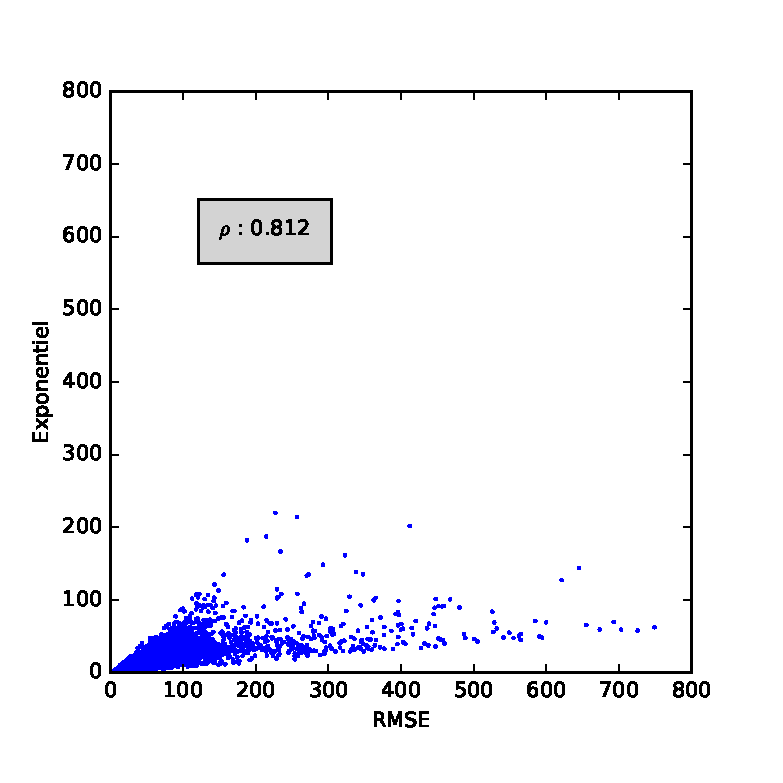
\includegraphics[width=7cm]{metrics-dist-exp.eps}}
   \caption{\label{fig:metrics-ann1}Comparaison entre le RMSE et le RMSE exponentiel pour chacune des prédictions.}
\end{figure}

\begin{figure}[h]
   \centerline{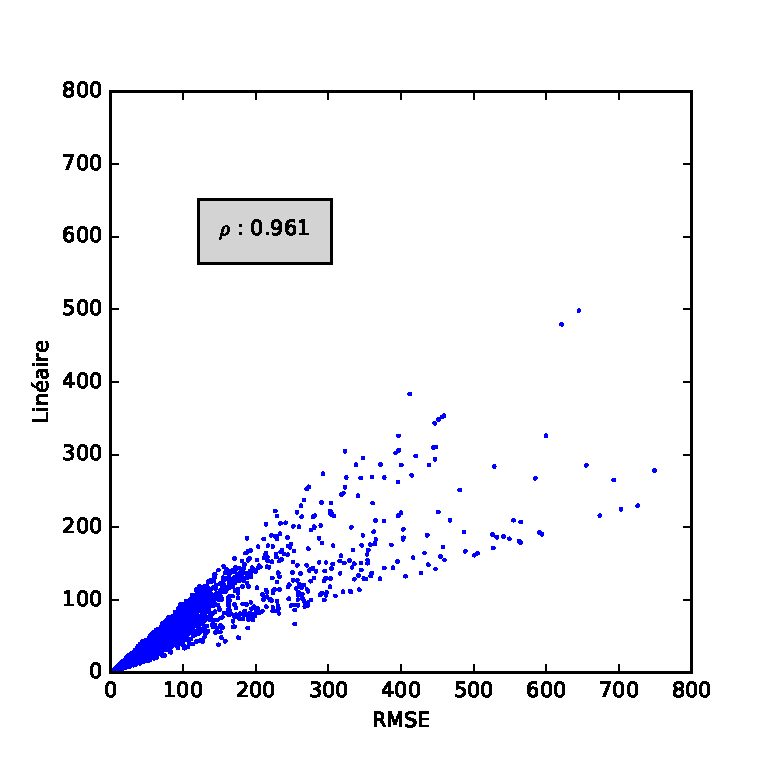
\includegraphics[width=7cm]{metrics-dist-lin.eps}}
   \caption{Comparaison entre le RMSE et le RMSE linéaire pour chacune des prédictions.}
\end{figure}

\begin{figure}[h]
   \centerline{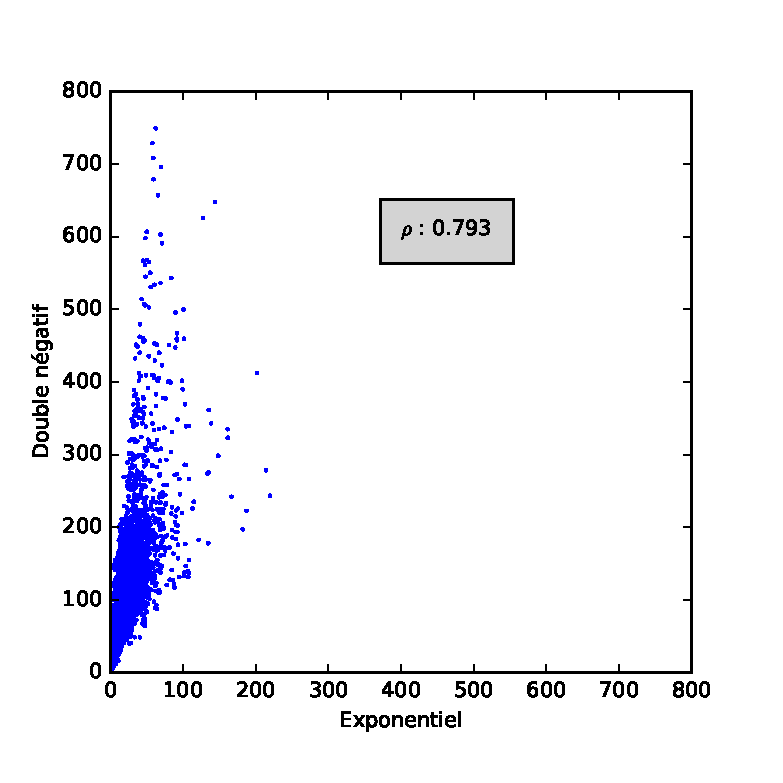
\includegraphics[width=7cm]{metrics-exp-double.eps}}
   \caption{Comparaison entre le RMSE exponentiel et le RMSE double négatif pour chacune des prédictions.}
\end{figure}

\begin{figure}[h]
   \centerline{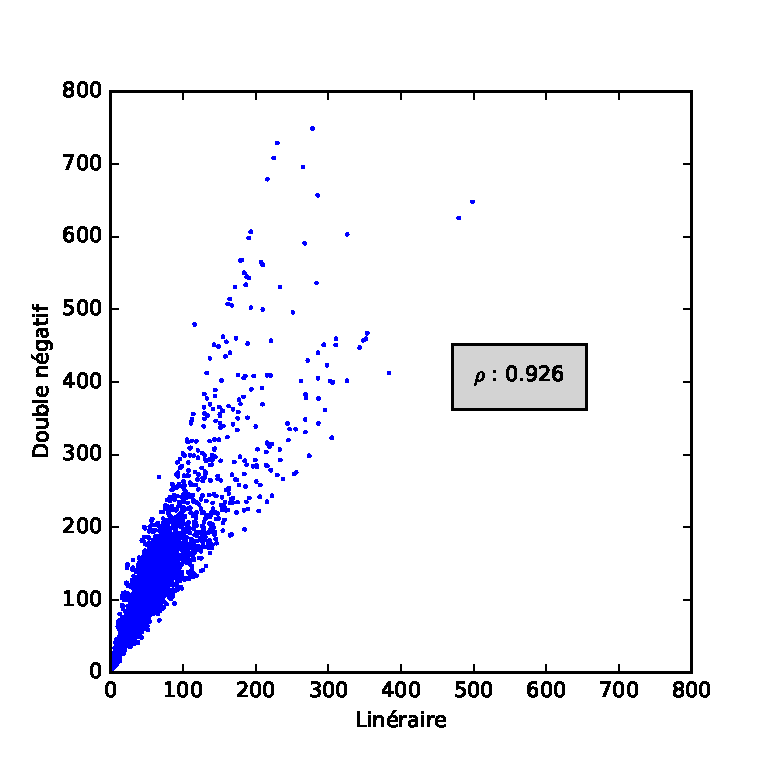
\includegraphics[width=7cm]{metrics-lin-double.eps}}
   \caption{Comparaison entre le RMSE linéaire et le RMSE double négatif pour chacune des prédictions.}
\end{figure}

\begin{figure}[h]
   \centerline{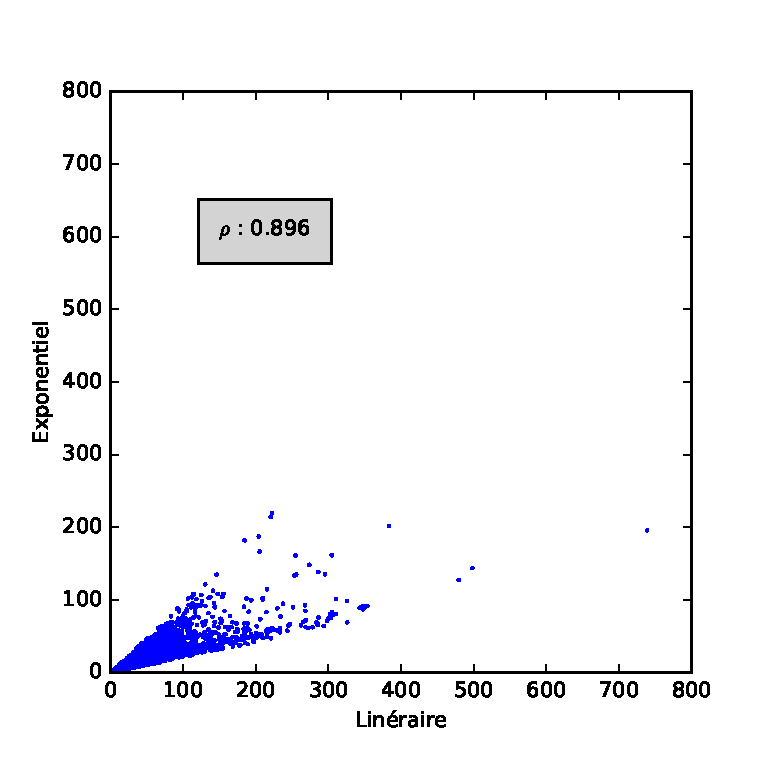
\includegraphics[width=7cm]{metrics-lin-exp.eps}}
   \caption{\label{fig:metrics-ann2}Comparaison entre le RMSE linéaire et RMSE exponentiel pour chacune des prédictions.}
\end{figure}


\FloatBarrier
\section{Résultats}

La figure \ref{fig:density} montre bien que la densité des trajets est plus élevée du côté ou la STIB a prédit une plus grosse erreur (à droite). On remarque aussi que côté droit garde une densité plus élevée que le côté gauche, même pour des points plus éloignés de la sécante. Cela montre que lorsque $k$NN se trompe, il se trompe peu, contrairement à la STIB.

\begin{figure}[h]
   \centerline{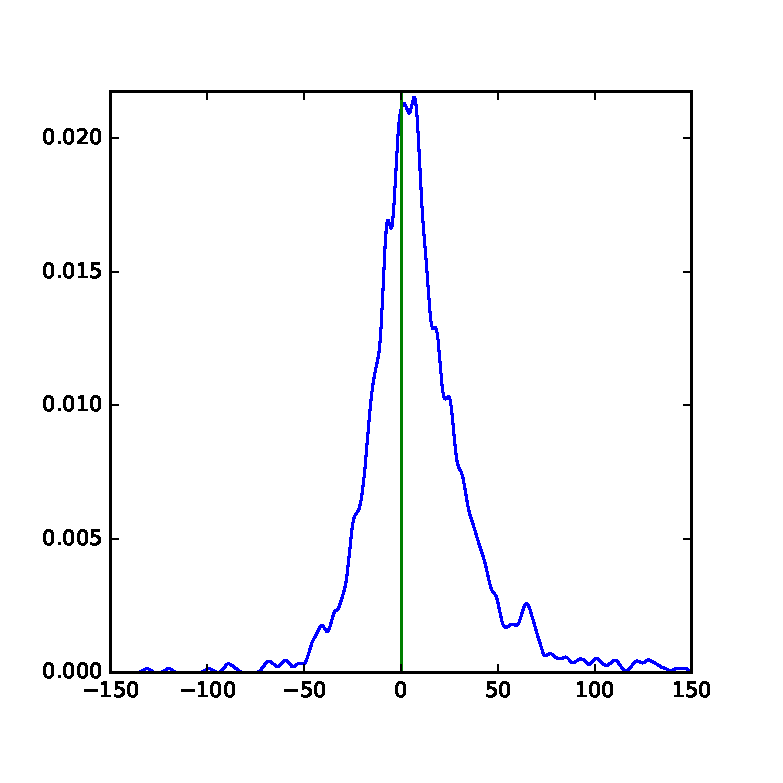
\includegraphics[width=9cm]{density.eps}}
   \caption{\label{fig:density} Densité des prédictions selon leur distance à la sécante pour la ligne du 95}
\end{figure}


\end{appendices}

\end{document}
